\def\qpmoy{%
	Quelle est la pression (moyenne globale ou inspiratoire) affichée sur le multimètre?
	\shortanswer[\cmh]%
	}

\begin{exercice}[Position de départ des contrôles]
De façon générale, la position midi (flèche du bouton alignée avec le curseur) correspond au réglage par défaut. Cette position devrait, en théorie,  pouvoir servir de réglage de départ pour débuter la ventilation de la majorité des patients. Il y a cependant plusieurs exceptions non négligeables à cette règle générale.

Cet exercice vise à vous faire explorer le comportement des différents paramètres en fonction de la position des contrôles.

\begin{itemize}
	\item Brancher l'appareil et installer un circuit et un poumon de test;
	\item Mettre le Monitron en fonction et positionner TOUT les contrôles à midi;
	\item Mettre la nébulisation en fonction;
	\item Ne pas démarrer la percussion.
\end{itemize}

	\exsection{PEP non oscillante}

	\posquestion{Quelle position du contrôle \param{Demande CPAP/PEEP}  désactive cette fonction, c'est à dire pas de pression positive continue (PPC)?}
	\posquestion{Quelle position correspond à une PPC de 5 \cmh ?}

	\posquestion{Quelle position correspond à une PPC de 10 \cmh ? }

	\exsection{Rapport \ie des percussions}
	\begin{itemize}
		\item Démarrer la percussion
		\item Régler le temps inspiratoire de la convection (basse fréquence) au maximum (sens antihoraire) et le temps expiratoire de la convection (basse fréquence) au minimum (sens horaire)
		\item Régler le contrôle \param{Débit pulsé} à 9h et le contrôle CPAP OSCILLANTE au maximum (sens antihoraire).
		\item Régler le Ti de la percussion le plus court possible
			(contrôle \param{Fréquence de percussion} en sens antihoraire).
	\end{itemize}

	\exsubsection{}

	Quelle est la pression (moyenne globale ou inspiratoire) affichée sur le multimètre?
	\shortanswer[\cmh]

	Pour chacune des interventions suivantes, prendre le temps d'observer l'apparence des percussions à chacune des vitesses de défilement du Monitron (1, 2, 5 et 8 s par écran)

	\begin{itemize}
		\item \posquestion {Tourner le contrôle RAPPORT i:e en sens horaire jusqu'à ce
	que le  rapport i:e affiché sur le Monitron soit de 1:1.1 (Ti $\approx$ Te).}
		\item Noter la position du contrôle. 
	\end{itemize}
	\qpmoy

	\begin{itemize}
		\item \posquestion {Tourner le contrôle RAPPORT i:e en sens horaire jusqu'à ce
	que le  rapport i:e affiché sur le Monitron soit de 1:1.5.}
		\item Noter la position du contrôle. 
	\end{itemize}
	\qpmoy

	\begin{itemize}
		\item \posquestion {Tourner le contrôle RAPPORT i:e en sens horaire jusqu'à ce
	que le  rapport i:e affiché sur le Monitron soit de 1:2.}
		\item Noter la position du contrôle. 
	\end{itemize}
	\qpmoy

	\exsubsection{}


	\begin{itemize}
		\item Régler le contrôle DEBIT PULSE à midi.
	\end{itemize}

	Quelle est maintenant la valeur du ratio \ie  affichée sur le Monitron ?
	\shortanswer

	\exsubsection{}

	\begin{itemize}
		\item Régler l'alarme de surpression du module de contrôle à la position la moins sensible (sens horaire).
		\item Régler les contrôles TEMPS INSPIRATOIRE et TEMPS EXPIRATOIRE à midi.
		\item Régler le contrôle CPAP OSCILLANTE au maximum.
		\item Régler le contrôle RAPPORT i:e à midi.
		\item Régler le contrôle DEBIT PULSE à 9h.
	\end{itemize}

	La courbe de pression devrait maintenant avoir l'apparence suivante :

	\centerline{\includegraphics{img/exr-controle1.pdf}}

	Quelle est la pression moyenne inspiratoire (affichée sur le multimètre numérique du module de contrôle) ?
	\shortanswer{\cmh}

	\posquestion{%
		\begin{itemize}
			\item Régler le contrôle RAPPORT i:e de façon à ce que la courbe de pression aie l'apparence suivante (ci-bas) et noter la position du contrôle. 
		\end{itemize}
		}

		\centerline{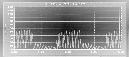
\includegraphics{img/exr-controle2.pdf}}

		Quel est le rapport i:e affiché par le Monitron ? \shortanswer{\cmh}

		Quelle est la pression moyenne inspiratoire (affichée sur le multimètre numérique du module de contrôle) ?

		\shortanswer{\cmh}
\end{exercice}
